\section{Problem setting}
\paragraph{Forward model}
Let  $\state_t\in \statesp \subset \mathbb{R}^{D_{\state}}$ for each $t=0,1,2,\ldots,T$ be a sequence of states, with $\state_0=\statest_0$ known.
The state dynamics arise from recursive application of a \emph{forward operator} \(\op{P}:\statesp\times  \forcingsp \to \statesp\) whose action is known conditional on an unknown time-invariant parameter, \(\forcing\in\forcingsp\subset \mathbb{R}^{D_{\forcing}}\), such that
\begin{align*}
    \state_{t}=\op{P}(\state_{\tm}, \forcing),\quad t=1, 2, \cdots, T.\numberthis\label{eq:ts-sem}
\end{align*}
Formally, we allow \(\op{P}\) to be stochastic, which we can make explicit by adding an unobserved white noise \(\vrv{\nu}_{t}\) to the arguments of $\op{P}$.
Equivalently, we may express a likelihood over current states given previous states and parameter. That is, there exists some nonnegative and appropriately normalised $f$ such that for each $t = 1,\ldots,T$,
\begin{equation}
\begin{aligned}
    \state_{t}&=\op{P}(\state_{\tm}, \forcing, \vrv{\nu}_{\tm}),  \\
    \iff p(\statest_t \gvn \state_{t-1}, \forcing) &= f(\statest_t; \state_{t-1}, \forcing).
\end{aligned}
\label{eq:ts-sem-stoch}
\end{equation}

The techniques that are available and suitable for inference depend on the degree to which the forward model is known.
We distinguish between two degrees of such knowledge.
If we may evaluate $f$ and its derivatives at any point,
or we can evaluate $\op{P}$ and its derivatives at any point, we call the forward model a \emph{white-box} model.
If we can evaluate only $\op{P}$, we call the forward model a \emph{black-box} model. 
Note that we assume the state dynamics has the Markov property, so that the likelihood factors as
\begin{align*}
    p(\statest_1, \ldots, \statest_T \gvn \forcing ) &= \prod_{t=1}^T p(\statest_t \gvn \state_{t-1}, \forcing) p(\forcing). \numberthis \label{eq:likelihood}
\end{align*}


\paragraph{Discrete bases} In the physical problems that motivate our approach, vectors possess an interpretation as a finite dimensional representation of a physical system of interest, as the coefficients of a projection of the system onto an orthogonal basis.
For example we could have \(\state_{t}\) represent instantaneous, discretised density and velocity field of a fluid distributed over some spatial domain, \(\op{P}\) the discretised forward predictor of a noisy fluid simulation, and the parameter $\forcing$ an inhomogenous forcing term arising from an external driver applied to the system. 
Such a finite representation is consistent with the way in which state dynamics are typically manipulated in machine learning settings (such as~\S 2.2 of~\citet{RasmussenGaussian2006}), where inference over finitely many evaluations is of primary concern.
Although the forward operator and vector space are both assumed to arise from some discretisation of a continuous-time, continuous-space system, we do not concern ourselves with the details of discretisation here. Instead, we assume that the discretisation error may be made negligible if the problem is discretised to a ``fine-enough basis'' e.g.~\cite{LassasDiscretizationinvariant2009}, for which it is necessary that we can handle high-dimensional state vectors.
In the examples here the bases are finite-element bases of top hat functions (Appendix~\ref{app:basis-functions}).

\paragraph{Bayesian inference} A Bayesian probabilistic model represents the quantities of interest with random variables by assigning some probability measure over the state space.
We represent our \emph{prior} belief (before observing any data) over plausible values that the parameter $\forcing$ can take using probability. 
An appropriate choice of prior measure regularises our inference towards some plausible region of solution space.
We place a prior probability density function over $\forcing$ and write $p(\forcingst)$ for the evaluation of such a density. 
For concreteness, we take the prior $p(\forcingst)$ to be a multivariate Gaussian, however the methods we discuss may utilise more general priors.
That is, the parameter prior satisfies
\begin{align*}
\forcing \sim \dist{N}(m_0,\mm{K}_0),
\end{align*}
where $\mm{K}_0 \in \mathbb{S}^{D_{\forcing}}_+$ is a PSD covariance matrix and $m_0 \in \mathbb{R}^{D_{\forcing}}$ is a mean vector.

Our goal is to sample values of the parameter $\forcing$ given the observations  \(\set{D}_T=\{\state_1=\statest_1, \cdots, \state_T=\statest_T\}\). That is, we seek to approximately compute, sample from, or otherwise describe (some property of) the \emph{posterior}
% We approach this in a probabilistic setting where both estimands and observations may be random variables.the posterior
\begin{align*}
    p\big( \forcingst \gvn \mathcal{D}_T \big) =  \frac{p(\forcingst) p(\mathcal{D}_T \gvn \forcingst)}{p(\mathcal{D}_T)},\numberthis \label{eq:bayes_rule}
\end{align*}
where the likelihood $p(\mathcal{D} \gvn \forcingst)$ admits a factorisation via~\eqref{eq:likelihood}.


\iffalse
For compactness we  define \(\forcing_{t}:=\forcing\gvn (\state_{0}{=}\statest_{0},\dots,\state_{t}{=}\statest_{t})\), and note that
% \russ{I can't see this factorisation --- does it rely on a kind of Bayes' rule?}
\begin{align*}
% \left(\forcing\gvn \state_{0}{=}\statest_{0},\dots,\state_{t}{=}\statest_{t}\right)
% &= \left(\left(\forcing\gvn \state_{0}{=}\statest_{0},\dots,\state_{\tm}{=}\statest_{\tm}\right) \gvn\state_{\tm}{=}\statest_{\tm},\state_{t}{=}\statest_{t}\right)\\
p(\forcing_{t})
&= p\left(\forcing_{\tm}\gvn
\state_{\tm}{=}\statest_{\tm},
\state_{t}{=}\statest_{t}
\right).\numberthis\label{eq:filtering}
\end{align*}
For a derivation of this rule, see Appendix~\ref{app:conditioning-dag}.
\fi

% The dynamical systems we study are of the following form:
% At each time \(t\), the system state is some spatial field  \nb{we may need to be slightly more general and include both observed and unobserved state} 
% Suppose we have a deterministic forward operator,
% \(\op{P}:\statesp\times  \forcingsp \to \statesp\) that maps a temporally evolving process from forcing space \( \forcingsp\) and state space \(\statesp\) at time $t-1$ to state space \(\statesp\) at time $t$, and where each of \(\statesp,\forcingsp\) is a (possibly random) vector space.
% Recursive application of the forward operator using
% \begin{align*}
%     \statest_{t}=\op{P}(\statest_{\tm}, \forcingst)
% \end{align*}
% defines a time series, ${\statest}_{0:T} = (\statest_0, \statest_1, \cdots, \statest_T)$.


% If we introduce randomness into this system, for example by allowing forcings, initial conditions to be random, or a random perturbation to the forward operator, then we write this as a random series, $\state_{0:T} = (\state_0, \state_1, \cdots, \state_T)$.

% \emph{Inverse problems} in this context are problems of the following sort:
% Assume the initial state is some random  \(\state_0\sim \pi\) and unobserved, can we estimate it from a realisation of the time series, \(\state_{1:T} = \statest_{1:T}
% \)?
% We will assume a  a prior \(\pi\) over \(\state_{0}\) encodes our  beliefs about the qualities of solutions, favouring, e.g. smoothness.

% Our method defines a coupled Gaussian Process representation of input and output fields\nb{cite some spatial GP people}, and then exploits the pathwise updates~\cite{WilsonEfficiently2020} to sample from the model posterior.
% Finally, ensemble data assimilation~\cite{EvensenData2009,RothEnsemble2017} accumulates updates from multiple timesteps.

\paragraph{Bayesian network and recursive updates} Recursive application of the forward operator
\begin{align*}
\state_{t} 
% \gvn \state_{\tm},\forcing 
&= \op{P}(\state_{\tm},\forcing ), \quad t=1,\cdots,T,
\numberthis \label{eq:proc_proj_sem_inv}
\end{align*}
given some known initial state \(\state_{0}=\statest_0\), defines a time series of random vectors, $\state_{1:T} := (\state_1^{\top}, \ldots, \state_T^{\top})^{\top}$. 
% \russ{Are we limited to first order Markov...?}
% \danm{most of the physical ones are first order markov, but they include the "velocity" in the state, so they are first order markov but only in the sense that physics itself is...}%That is a real good question. I... don't think we are limited to first order markov, but the way it's written there does restrict it to first order markov. OTOH first order markov gets us much. We can talk about packing hitsory together to make a higher order markov thing. Does that preclude most SPDEs? I don't think so, most of the physical ones are first order markov, but they include the "velocity" in the state, so they are first order markov but only in the sense that physics itself is. Unless we've written something that implies otherwise?} 
% \russ{Maybe we could write a sentence to this effect}
% \danm{rolled it into the example, how about that?}
The corresponding Bayesian network, depicted in Figure~\ref{fig:ts_dag}, defines a simple dependence structure between field-valued variates, although \emph{within} a (vector-valued) variate we permit arbitrary dependencies between sites.

\subfile{bayesnet}

Except in a small number of cases, the distribution induced by this definition has no closed form representation. 
A notable exception is the case in which Gaussian distributions are perturbed by linear operators, resulting in another Gaussian distribution~(\citealp{RasmussenGaussian2006}~\S~2.2; \citealp{solak2002derivative}; \citealp{ghosal2006posterior}~Theorem~5).
\russ{Broken references?}

We can use the independence structure of the variates to iteratively update posteriors at time $T-1$ into posteriors at time $T$ by conditioning on successive observations, since
\begin{align*}
    &\phantom{{}={}} p(\forcingst \gvn \mathcal{D}_{t}) \\
    &= p(\forcingst \gvn \mathcal{D}_{t-1} ) \frac{ p(\mathcal{D}_t \gvn \mathcal{D}_{t-1}, \forcingst)}{p(\mathcal{D}_t)} \\
    &= p(\forcingst \gvn \mathcal{D}_{t-1} ) \frac{ p(\statest_t \gvn \state_{t-1}, \forcingst)}{p(\mathcal{D}_{t-1})\int p(\statest_t \gvn \state_{t-1}, \forcingst') p(\forcingst') \, d\forcingst'}.
\end{align*}

%\russ{Can this equation be converted into the same $p(\cdot)$ notation used in Appendix~\ref{app:conditioning-dag}?}
%\danm{yes we can convert this to density notation, although the posterior update never evaluates a density, so it feels more ``natural'' to to keep it in terms of RVs, since the gaussian density is fictitious anyway. Or?}
%\russ{ I do not understand the equation here, or its relevance to Appendix~\ref{app:conditioning-dag}.}
%\danm{OK, needs bridging text then}
%\russ{Is it intentional that we are condition on $\state_{t-1}$ twice?}
%\danm{Yes, intentional but maybe more confusing that I was imagining. At each time step we evaluate based on two timesteps simulataneously; since one of them has already been assimilated the double conditioning ``does nothing''. If that sounds confusing shouyld revisit.}
%\russ{I realise my brain was not working. After changing the notation around, this statement is obvious.}
Unfortunately, computing the posterior even using recursive updates is usually intractable.
The %pushforward measure (i.e. 
probability measure of the random variable $\state_t = \op{P}(\state_{t-1}, \forcing)$  can be arbitrarily complicated, and thus the posterior~\eqref{eq:bayes_rule} induced by \eqref{eq:proc_proj_sem_inv} will typically be intractable.
% The normalising constant $p(\mathcal{D}_t)=\int p(\mathcal{D}_t \gvn \forcingst') p(\forcingst') \, d\forcingst'$ is the source of intractability.
Popular approaches for estimating/approximating the posterior distribution in the absence of the normalising constant are to either: (i) use sampling algorithms like Markov Chain Monte Carlo (MCMC) and importance sampling (IS)); or (ii) impose a particular parametric distribution on the posterior (e.g. variational inference and Laplace approximations).
We leverage both in what follows.

\paragraph{Example} For concreteness we use a specific example throughout this paper, illustrated in  Figure~\ref{fig:dynamicalsystem}.
The forward operator $\op{P}$ applies incompressible Navier-Stokes fluid flow forward-propagation equations on a square domain.
The state $\state_t$ of the system is by assumption completely characterised by a discretisation of the problem into a locally-constant \(256\times 256\) lattice of cells, each of which possesses a density (\ref{fig:states}) and two-dimensional velocity (not shown) for an overall state dimension of \(D_{\state}=256\times 256 \times (1+2)\).
The latent parameter $\forcing$, a discretised 2-vector field, is characterised completely by a vector of dimension \(D_{\forcing}=256\times 256 \times 2\).

\begin{figure*}[h!t]
     \centering
    \begin{subfigure}{0.7\textwidth}
        \centering
        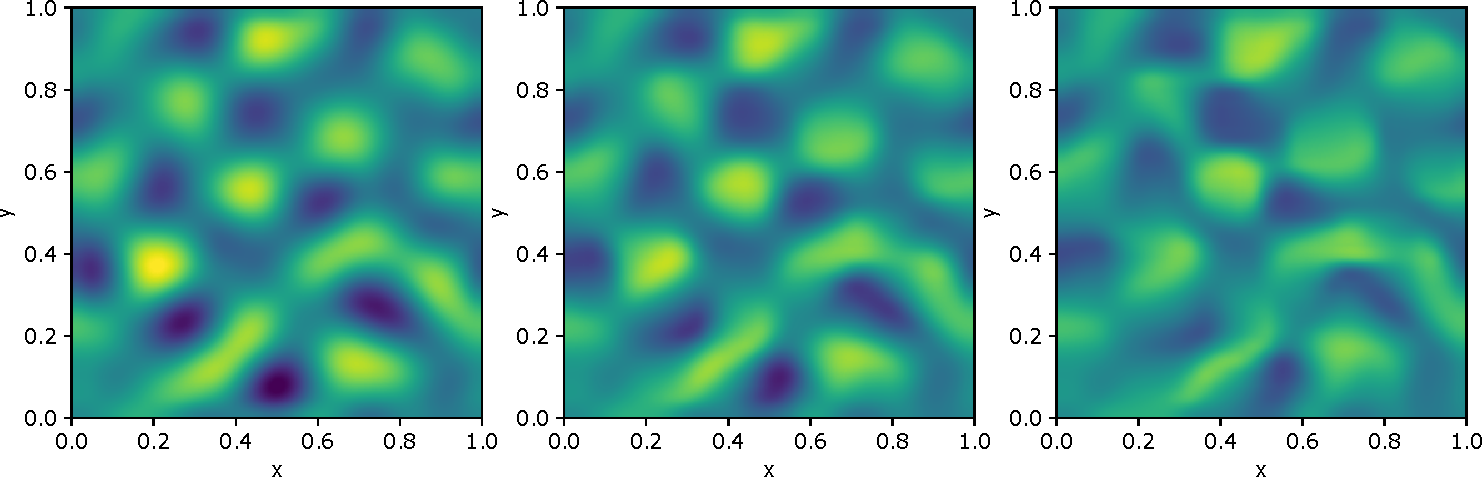
\includegraphics[scale=0.35]{ns_p_trim.pdf}
         \caption{From left to right, states (in this case, density fields) $\state_{0}, \state_{1}, \state_{2}$ evolving through time.}
         \label{fig:states}
     \end{subfigure}
     \begin{subfigure}{0.25\textwidth}
         \centering
        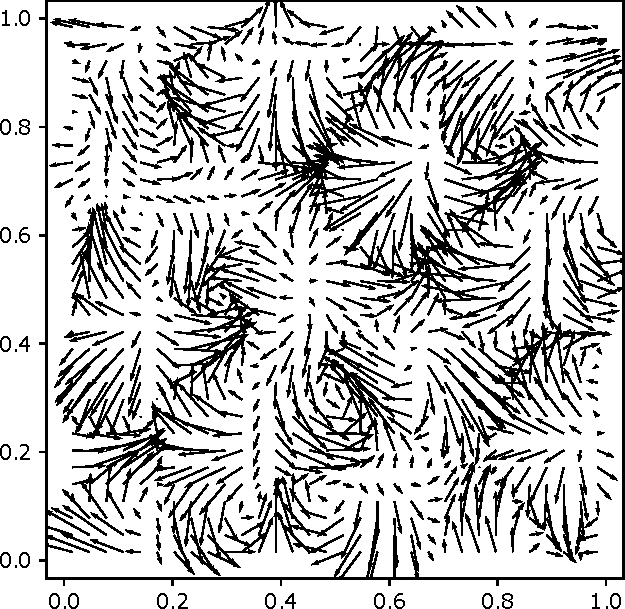
\includegraphics[scale=0.25]{ns_force_trim.pdf}
         \caption{Unobserved parameter $\forcing$.}
         \label{fig:forcing}
     \end{subfigure}
     \hfill
    \centering
    \caption{An example Navier-Stokes fluid flow system, used as a case study in this work. State and velocity vectors are projected into the original space representing the evolutions of a physical system.}
    \label{fig:dynamicalsystem}
\end{figure*}


% \section{Deterministic operator inversion}
\section{Approaches to model inversion}
We review some classical approaches to model inversion in \S \ref{sec:InversionMAP} - \S \ref{sec:InversionGP}, then present our new approach, \meth{}, in \S \ref{sec:EnsembleInversion}, and discuss hyperparameter selection in \S \ref{sec:HyperparamSelection}.

\subsection{Inversion by optimisation}\label{sec:InversionMAP}
One straightforward approach is to choose by optimisation a parameter estimate that minimises some discrepancy between the observation and the model prediction given the parameter, minimising some prediction loss. 
If this loss arises from an observation likelihood we can frame this as likelihood maximisation.
Any 
%(not necessarily unique)
\emph{maximum a posteriori} (MAP) estimate $\hat{\forcingst}$ satisfies
\begin{align*}
    \hat{\forcingst} \in \argmax\limits_{\forcingst \in \mathcal{U}}  \log 
         p\big( \forcingst \gvn \mathcal{D}_t \big)
         + \log p(\forcingst).\numberthis \label{eq:pred_error_inv}
\end{align*}
\russ{This looks possibly wrong? Shouldn't the first term be a log likelihood? Also a negative sign?}

\iffalse
In the case where only a black-box forward model is available, we may obtain a summary of the posterior through simulation \textcolor{red}{see section} and then apply the estimate~\eqref{eq:map_estimate}.
Alternatively, given some discrepancy measure $L$, we may minimise the discrepancy between ground-truth observations and predictions of the forward model,
\begin{align*}
    \hat{\forcingst} :=\argmin_{\forcingst}
        \sum_{t=1}^T L\left(
            \statest_{t},
            \op{P}(\statest_{\tm}, \forcingst )
        \right).\numberthis \label{eq:pred_error_inv}
\end{align*}
\fi

The optimisation problem described in (\ref{eq:pred_error_inv}) is often under-determined, in the sense the optimum may not be unique. 
To make matters worse, gradient-based optimisation may converge to local, rather than global, maxima.
When the dimensionality $D_{\forcing}$ is large, traditional second order optimisation methods can become computationally intractable on account of the large linear systems that need to be solved.
Additionally, if the log-likelihood is non-convex in $\forcing$, most algorithms will only be able to find a local optimum of~\eqref{eq:pred_error_inv}.
Under certain conditions~\citep[Chapter 5]{WrightOptimization2021}, stationary points of~\eqref{eq:pred_error_inv} may be efficiently computed, even for high dimensional $D_{\forcing}$, by gradient descent or stochastic gradient descent~\citep{XuADCME2020,MacKinlayModel2021} of the negative log-likelihood function for a white-box forward model.
A downside of point estimates obtained by optimisation, is that they do not contain any uncertainty estimates for given solutions.
Efficient routines exist for computing uncertainty of point estimates via second order methods that exploit sparsity and variable ordering heuristics~\citep{DellaertFactor2017}, however an optimisation-based perspective is inherently limited to uncertainty quantification locally around the MAP estimate.

In the Bayesian setting, we can remedy issues associated with both non-convexity and lack of uncertainty information, using appropriate prior $p(\forcing)$ in~\eqref{eq:pred_error_inv} to regularise solutions towards \emph{a priori} plausible solutions, and assigning a posterior weight to various candidate solutions.
In the pure optimisation setting, we can also use regularisation to penalise the parameter-space towards plausible solutions, although inclusion of the regularisation term loses the intuitive interpretation that we gain from employing a prior.
%However, excessively large prior regularisation terms can lead to undesirable properties of the estimate, such as slower convergence to a true model parameter in the case of a well-specified model.

\iffalse
This approach can be generalised to a stochastic forward operator, by taking expectations
\begin{align*}
    \hat{\forcingst} :=\argmin_{\forcingst}
        \Ex_{\vrv{\nu}}[L\left(
            \statest_{t},
            \op{P}(\statest_{\tm}, \forcingst,\vrv{\nu})
        \right)].\numberthis \label{eq:pred_error_inv_stoch}
\end{align*}
Solution in that case may be estimated by stochastic gradient descent method. \russ{Monte Carlo gradient method == SGD and friends?}\danm{yes, but need to expand if we keep this bit in there.}
\fi 

%\subsection{Naive Bayesian inversion}
%\label{sec:naive_bayes}

%\russ{I still don't understand the construction. Maybe my confusion is related to the lack of subscripts on $\mathsf{z}$ and $\mathsf{u}$, or maybe not. I general I cannot see how $\mathsf{z}$ is a Gaussian process is compatible with~\eqref{eq:proc_proj_sem_inv} holding. Maybe my confusion is related to what ``simple choice for probabilistic modelling" means. Maybe my confusion is related to whether $\mathsf{z}$ is Gaussian when indexed by time, space or both?}




\subsection{Bayesian inversion with linearised Gaussian processes}\label{sec:InversionGP}
\label{sec:error_prop}
\iffalse
A pragmatic choice for probabilistic modelling of the random functions $\state$ and $\forcing$ is to approximate all steps by a multivariate Gaussian, where for some mean \(\vv{m}(\state_{\tm},\forcing)\) and covariance \(\mm{K}_{\state}(\state_{\tm},\forcing )\) functions, for all $t = 1, \ldots, T$,
\begin{align*}
p(\state_{t} \gvn \state_{\tm}, \forcing)
%\gvn \state_{\tm},\forcing
&\approx \dist{N}(\vv{m}(\state_{\tm},\forcing), \mm{K}_{\state}(\state_{\tm},\forcing ))
\numberthis \label{eq:gaussian_approx_proc}.
\end{align*}
This is appropriate for deterministic white-box forward operators.
% This presumes that there exists some mean function \(\vv{m}(\state)\) and covariance function \(\op{K}(\state)\) such that the forward predictive density is well approximated by the pushfoward of the forward predictor \eqref{eq:proc_proj_sem_inv}.

Choice of \(\vv{m}(\state_{\tm},\forcing) \) and \(\mm{K}_{\state}(\state_{\tm},\forcing)\) may be motivated by different senses in which we approximate the target distributions, each leading to different algorithms for inference, with different tradeoffs of accuracy and computational cost.

% It is the strategic selection of these choices which is at the core of this paper.
%\russ{Are~\eqref{eq:proc_proj_sem_inv} and~\eqref{eq:proc_proj_sem_inv} saying the same thing if certain operators/initial conditions are allowed to be stochastic? My preference is for notation~\eqref{eq:proc_proj_sem_inv} because then we would not need to know what a ``conditional random variable" is, if there is such a thing.}
% Typically we  assume the mean function is given by the forward predictor \(\op{M}_{\state}(\state_{\tm},\forcing)=\op{P}(\state_{\tm},\forcing )\) but other models are are possible.\nb{if we don't get to Laplace approx skip this}

% We define
% \begin{align*}
%     \state_{t}&:=\proj_{\vv{S}}\state_t.
% \end{align*}
% We additionally use a ``free'' projection \(\proj_{\vv{x}}\) where we may vary \(\x\).
% As mentioned at the beginning of the section, we restrict attention to the problem where the forcing \(\forcing\) is entirely unobserved and is the primary focus of inference.~\footnote{The derivations are similar if, for example, we wish to estimate initial conditions \(\state_{0}\).}
% The forcings are unobserved, \(\seeninp{}:\forcing \mapsto \emptyset\).\nb{Wrong! we need this projection to define the fucntion completely, i.e. be a parameterisation rather than a projection}
% We choose a possibly different vector of test points \(R\) to define \(\seenstate{}:=\proj_{\vv{Y}}\), the projection used in the forward prediction.\nb{should have raised this possibility earlier?}

% \(\forcing,\state_{t}\gvn \state_{\tm} \) are not in general conditionally jointly Gaussian,
% We introduce an additional assumption,
% that there is some \(\state_{\tm}\)-conditional linear relationship such that for \(s\in\set{S}\),
% \begin{align*}
% \left.\left[\begin{array}{c}
%     \state_{t} \\
%     \forcing(s)
% \end{array}\right]\right|\state_{\tm}{=}\statest_{\tm}
% &\sim\dist{N}\left(
%     \left[\begin{array}{c}
%         {m}_{\state_{t}}\\
%         {m}_{\forcing}
%     \end{array}\right],
%     \left[\begin{array}{cc}
%         \mm{K}_{\statest\statest}
%         & \vv{k}_{\statest\forcing} \\\ % 3 backslashes or it breaks for some reason
%           \vv{k}_{\statest\forcing}^{\top}
%         &k_{\forcing\forcing}
%     \end{array}\right]
% \right).
% \end{align*}
% where
% \begin{align*}
%     {m}_{\state_{t}}&=\Ex\state_{t}\gvn \state_{\tm}{=}\statest_{\tm}\\
%     m_{\forcing}&=\Ex\forcing(s)\gvn \state_{\tm}{=}\statest_{\tm}\\
%     \mm{K}_{\statest\statest}&:=\cov(\state_{t},\state_{t})\gvn \state_{\tm}{=}\statest_{\tm}\\
%     % k_{\statest\forcing}(s)^{\top} &= (k_{\statest_1 \forcing}(s), \cdots, k_{\statest_{|S|}\forcing}(s))\\
%     k_{\statest_i \forcing} &:=\cov(\state_{t},\forcing(s))\gvn \state_{\tm}{=}\statest_{\tm}\\
%     k_{\forcing\forcing}&:=\var(\forcing(s))
% \end{align*}
% % $\proj_{s_i}\state_{t}$ denotes the $i$th element of the projection of $\state_{t}$ using $\proj_{\vv{S}}$.
% the finite dimensional distributions are given
%  \(\forcing\sim \mathcal{N}({m}_{\forcing},\mm{K}_{\forcing\forcing})\) with \(\mm{K}_{\forcing\forcing}\) having $i,j$th element $k_{\forcing\forcing}(x_i,x_j)$.
% The joint finite-dimensional distributions are
\fi

Our goal is to approximate the posterior $p(\forcingst \gvn \mathcal{D}_t)$ using a Gaussian distribution $q(\forcingst \gvn \mathcal{D}_t)$ that admits an iterative update in terms of $q(\forcingst \gvn \mathcal{D}_{t-1})$.
To this end, define
\begin{align*}
    q(\forcingst \gvn \mathcal{D}_{t}) := \mathcal{N}(m_t, \Sigma_t) \approx p(\forcingst \mid \mathcal{D}_t), \numberthis \label{eq:approx_distribution}
\end{align*}
where $m_t \in \mathcal{U}$ and $\Sigma_t \in \mathbb{S}^{D_{\forcing}}_+$ are mean and covariance parameters. 
We take $q(\forcingst\gvn\mathcal{D}_0)$ to be the (exact, unconditional) prior, $q(\forcingst\gvn\mathcal{D}_0)=p(\forcingst)$.

\paragraph{Linearisation of the forward operator} A classic choice is to define the mean and covariance parameters in terms of a linearised approximation to the forward operator of the system, \( \op{P}\).
This is the basic technique underlying the propagation of errors, the Extended Kalman Filter, and more generally, Gaussian Belief propagation  (e.g.~\citet{OrtizVisual2021}).
Specifically, for some expansion point \(\forcingst_0\), we make the linear approximation
\begin{align*}
    \state_t = \op{P}(\state_{\tm}, \forcing)
    &\approx\underbrace{
    \op{P}(\state_{\tm},\forcingst_0)
    + %\begin{bmatrix}
        % \mm{J}_{\state_{\tm}}\\
        \mm{J}_{\forcingst_0}
    % \end{bmatrix}
    % \begin{bmatrix}
        % \statest-\statest_{0}\\
        (\forcing-\forcingst_0)}_{:= \widehat{\op{P}}_{\forcingst_0}(\state_{\tm}, \forcing)},
    % \end{bmatrix},
    \numberthis \label{eq:linear_p}
\end{align*}
where
\begin{align*}
    % \mm{J}_{\state_{\tm}}&:=\left[\nabla_{\statest}\op{P}(\statest,\forcingst)\right]_{\statest=\state_{\tm}, \forcingst=\forcingst_0}\\
    \mm{J}_{\forcingst_0}&:=\left.\nabla_{\forcing}\op{P}(\state_{\tm},\forcingst)\right|_{\forcingst=\forcingst_0}.
\end{align*}
% are the Jacobian matrices associated with each argument.
% Collectively these motivate an approximate update rule.
%We use the linearised form \eqref{eq:linear_p} to approximate \eqref{eq:gaussian_approx_proc}, expanding about the prior mean
\paragraph{Approximation of the joint conditional}
We use the linearised form \eqref{eq:linear_p} to define the approximate conditional distribution of $\state_t$ and $\forcing$ given $\mathcal{D}_{t-1}$.
Setting 
\(\forcingst_0=
m_{\tm}\), in this approximation, we find that the joint conditional distribution satisfies
\begin{align*}\left.
    \begin{bmatrix}
        \forcing \\ \state_{t}
    \end{bmatrix}\right| \mathcal{D}_{t-1}
    &\approxdisteq \left.
    \begin{bmatrix}
        \forcing \\
        \widehat{\op{P}}_{m_{t-1}}(\statest_{\tm},\forcing) +\vrv{\varepsilon}
    \end{bmatrix} \right| \mathcal{D}_{t-1} \numberthis\label{eq:ekf-linearisation}
\end{align*}
where \(\vrv{\varepsilon}\sim \dist{N}(0,\sigma^2\mm{I}\)) is a noise term that admits a degree of model misfit.
%\russ{Minor for now, and hard to chat about over text. Looking at~\eqref{eq:discrete_joint_enkf_sim}, if the $\sigma^2 I$ term is only added to the ``likelihood'' i.e. the upper left block of the covariance, wouldn't this be modelling a variance in the observation (aleatoric). If the $\sigma^2 I$ term is added to the top left and bottom right blocks, it would be an uncertainty in the model prior (epistemic). Is this the same as model misfit? Or maybe I am reading this wrong because some of these variables are $Z$ and some are $U$?}
%\danm{Hmm. Your observation \sout{possibly} fixes a bug that i've been looking at the code.}
%\danm{Was I overthinking it? Adding epistemic noise ... is that simply by adding  i.i.d noise to the U deviations? looks like it.} \danm{or inflate the posterior deviations equivalently to adding noise. TBC in \ref{sec:u-uncertainty}} 
% \danm{maybe this section is pointless? Will it even be used as a baseline?}

\paragraph{Updating the approximate posterior}
Under this approximation, the moments of the updated approximate density $q(\forcingst \mid \mathcal{D}_t)$ in the form \eqref{eq:cond-joint-normal} are given by
\begin{align*}
    {m}_{t}
        &= m_{t-1} + \emph{G} (\statest_t -  \widehat{\op{P}}_{m_{t-1}}(\statest_{\tm},m_{t-1})) \\
        \Sigma_t &= \Sigma_{t-1} - \emph{G}  J_{m_{\tm}} \Sigma_{t-1}
\end{align*}

\noindent where \( \emph{G} := \Sigma_{t-1}J_{m_{\tm}}^\top (J_{m_{\tm}} J_{m_{\tm}}^\top + \sigma^2 I)^{-1} \) is the gain matrix and the inverse is meant in a generalised sense. 
The gain matrix $G$ may not need to be formed explicitly, although linear systems involving the gain matrix need to be solved.
\iffalse
\begin{align*}
    {m}_{\state_{t}}
        &=\op{P}(\statest_{\tm},\vv{m}_{\forcingst})\numberthis\label{eq:linear-p-state-mean}\\
    \mm{K}_{\state_{t}\state_{t}}
         &=J_{{m}_{\forcingst}}\mm{K}_{\forcing\forcing}J_{{m}_{\forcingst}}^{\top} +\sigma^2\mm{I}\numberthis \label{eq:linear-p-state-cov}\\
    \mm{K}_{\state_{t}\forcing}
    % \mm{K}_{\statest\forcingst}{}
        &=\mm{K}_{\forcing\forcing}J_{{m}_{\forcingst}}^{\top}\numberthis \label{eq:linear-p-cross-cov}
\end{align*}
since \(\widehat{\op{P}}\) is linear.
% We can envisage this as a variational approximation, where the posterior mean and variance are chosen to minimise a KL-divergence between a true posterior and the local posterior approximation.\nb{write out KL-divergence version?}
This provides a recipe for iteratively updating beliefs about \(\forcing\) given new observation pairs \(\state_{\tm}{=}\statest_{\tm},\state_{t}{=}\statest_{t} \) by iteratively applying \eqref{eq:cond-joint-normal} to the moments arising from linearised approximation~\eqref{eq:ekf-linearisation}.
%Given some prior distribution for \(\forcing\) we can estimate \(\state_{t}\gvn (\state_{\tm}{=}\statest_{\tm},\forcing{=}\forcingst)\) using the linearised \eqref{eq:ekf-linearisation}, so that the observation likelihoods may be put into conditionally-jointly-normal form \eqref{eq:cond-joint-normal}, with moments given in terms of the Jacobian of the operator as per \eqref{eq:linear-p-state-mean}--\eqref{eq:linear-p-cross-cov}.
%Next, we can update our estimates for the posterior moments of \(\forcing\) by applying \eqref{eq:gaussian-cond-mean} and \eqref{eq:gaussian-cond-cov}.
\fi
This gives an update for the parameters $m_t$ and $\Sigma_t$ of $q(\forcingst \gvn \mathcal{D}_t)$ in terms of the parameters $m_{t-1}$ and $\Sigma_{t-1}$ of the previous density $q(\forcingst \gvn \mathcal{D}_{t-1})$ and observation $\statest_t$.

This approach can produce inferior results for problems where the action of the forward operator is not well-summarised by a linear transformation about the mean.
In practice for nonlinear models this means that the value of \(\sigma^2\) plays a role in reducing the influence of new observations and increasing the stability of updates.
Linearisation also performs unfavourably in high-dimensional problems.
The storage requirements of the  posterior statistics are large, comprising a mean function and also a covariance matrix between all sites, necessitating updating a \(D_{\forcing}\times D_{\forcing}\) covariance matrix. 
Further, computing this update can be  expensive, as the updates in \eqref{eq:gaussian-cond-var} and \eqref{eq:gaussian-cond-mean} require solving a linear system, which incurs a \(\mathcal{O}(D_{\vrv{\state}}^3)\) computational time cost.
Moreover, the capacity of this model to handle non-deterministic predictions is limited, since only linearly additive noise may be easily applied to the prediction model.
In the next section we attempt to address these problems simultaneously using an ensemble sampling method.

\subsection{Our solution: ensemble inversion via \meth{}}\label{sec:EnsembleInversion}

\begin{figure*}[h!t]
     % \centering
    \begin{subfigure}{0.3\textwidth}
         % \centering
        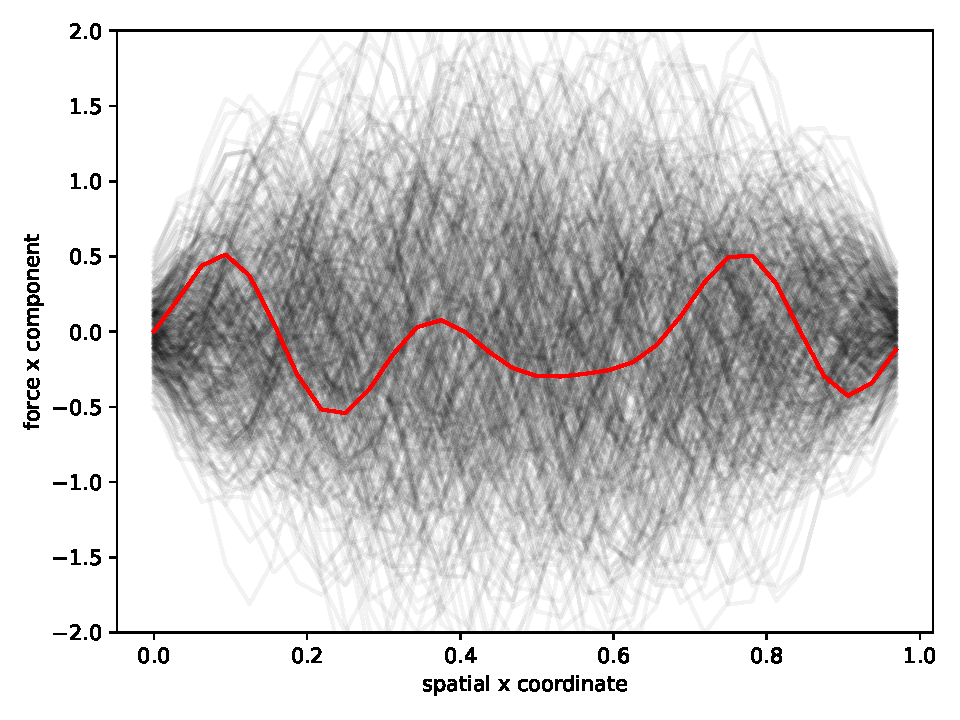
\includegraphics[scale=0.35]{meth_ex_guess_0.pdf}
         \caption{Prior samples of \(\forcing\)}
         \label{fig:meth_ex_0}
    \end{subfigure}
    \begin{subfigure}{0.3\textwidth}
         % \centering
        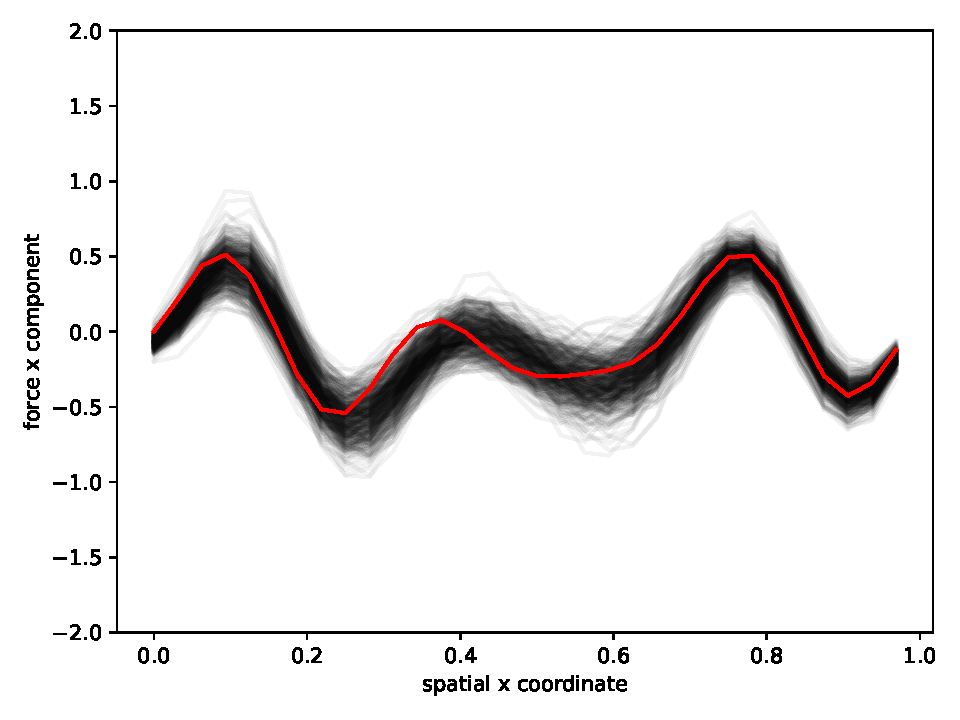
\includegraphics[scale=0.35]{meth_ex_guess_1.pdf}
         \caption{\meth{} samples \(\forcing\gvn \state_0,\state_1\).}
         \label{fig:meth_ex_1}
    \end{subfigure}
    \begin{subfigure}{0.3\textwidth}
         % \centering
        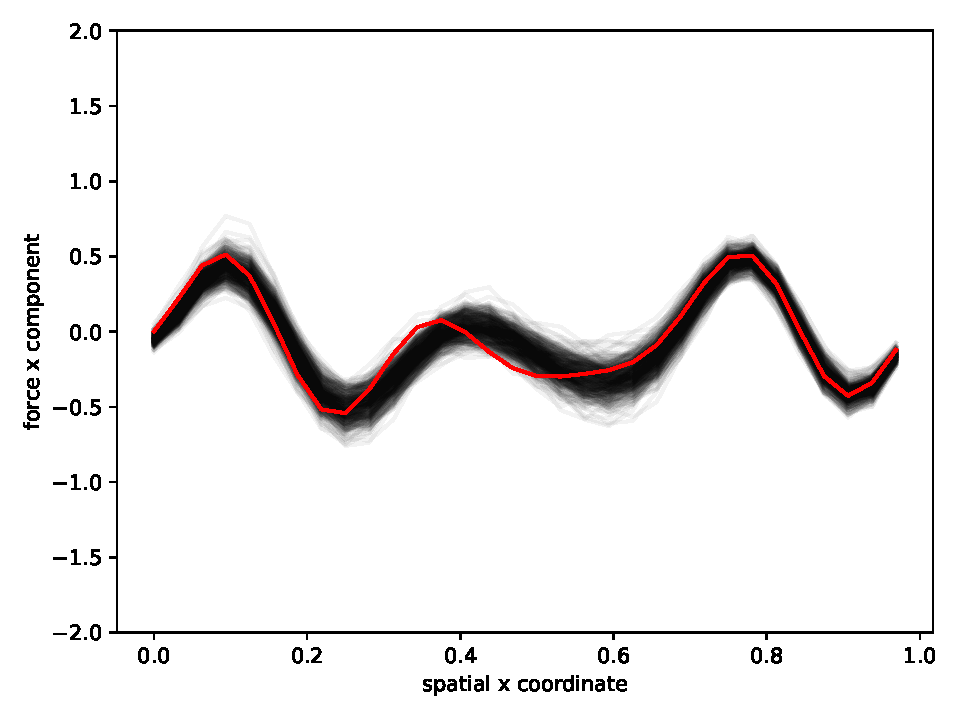
\includegraphics[scale=0.35]{meth_ex_guess_4.pdf}
         \caption{\meth{} samples \(\forcing\gvn \state_0,\cdots\state_5\).}
         \label{fig:meth_ex_4}
     \end{subfigure}
     \hfill
    \centering
    \caption{A slice along the \(x\) spatial  axis of  \(N=400\) sampled solutions computed via \meth{}. The solid red line shows ground truth, and each transparent grey line is one sample from the solution space.}
    \label{fig:inverse-slices}
\end{figure*}


The aforementioned limitations of the linearised propagation of errors can be eased by moving to Monte Carlo inference, wherein distributions are no longer summarised by their moments but  by samples drawn from those distributions.
Specifically, our method, \meth, is related to the family of Ensemble Kalman methods of Data Assimilation~\cite{EvensenData2009} and their generalisation to solve inverse problems~\cite{IglesiasEnsemble2013}.
Unlike the linearised version, ensemble methods are applicable to black-box models and stochastic models.  They summarise all random variates through an ensemble of (possibly approximate) samples from the distribution of that random variate.
The price for this is a need to execute the forward model more times (once for each ensemble member), with ensemble sizes typically in the order of hundreds.

In typical Gaussian inference we perform  an update by applying Bayes' rule to the distributions of the random variates involved, e.g. integrating the densities in~\eqref{eq:bayes_rule}, or in the case of conjugate models by updating moments of the belief distribution as per~\eqref{eq:cond-joint-normal}.
An ensemble-wise Gaussian eschews either of these in favour of perturbing the empirical distribution induced by samples in our ensemble.
That is, the \emph{empirical} ensemble moments satisfy the data-conditional update formula~\eqref{eq:cond-joint-normal}.
We use the Matheron update~\citep{WilsonPathwise2021} to perform the perturbation without evaluating the intermediate densities or forming covariance matrices.

Each sample from the prior belief distribution is perturbed so that the perturbed ensemble represents approximately independent samples from the posterior distribution conditional on the observations.
Such methods are frequently more computationally efficient and flexible than the error-propagation method of section \ref{sec:error_prop}, which acts directly upon the sufficient statistics of the Gaussian distribution rather than samples.
Further, ensemble methods are widely understood to attain superior performance in non-linear systems~\citep{FearnheadParticle2018}.
\meth{} is precisely the application of this method to the inference of hidden parameters rather than model states as in classical filtering.

%\russ{I think I am confused about what should be bold or not bold like $\forcing$ or $\forcingst$.}
%What is a random variable and what is a sample? https://stats.stackexchange.com/questions/368492/about-sampling-and-random-variables
\paragraph{Ensemble of parameters and states}
In  \meth{}, we begin by sampling from the prior distribution for \(\forcing \sim p(\forcingst)\) independently $N$ times.
We write the samples as
\begin{align*}
    \mm{U}_{0}= \begin{bmatrix}
        \forcingst_{0}^{(1)}, & \cdots, & \forcingst_{0}^{(N)}
    \end{bmatrix} \in \mathbb{R}^{D_{\forcing}\times N}.
\end{align*}


Our goal is to successively update this ensemble, constructing new ensembles  such that their columns contain samples from an approximate posterior $\forcing \sim \rho(\forcingst \gvn \mathcal{D}_t)\approx p(\forcingst \gvn \mathcal{D}_t)$. We similarly write such samples as
\begin{align*}
    \mm{U}_{t}=\begin{bmatrix}\forcingst_{t}^{(1)}, & \cdots, & \forcingst_{t}^{(N)} \end{bmatrix} \in \mathbb{R}^{D_{\forcing}\times N}.
\end{align*}
We now define the approximate posterior $\rho(\forcingst \gvn \mathcal{D}_t)$.  Mirroring the moment-centric approximation~\eqref{eq:approx_distribution}, we introduce an ensemble-centric approximation  with parameters replaced by empirical estimates of parameters,
$$\rho(\forcingst \gvn \mathcal{D}_t) := \dist{N}(\overline{\mm{U}}_t,\breve{\mm{U}}_t\breve{\mm{U}}^{\top}_t+ \tau^2\mm{I}) \approx p(\forcingst \gvn \mathcal{D}_t), $$
where empirical means and empirical variances are
\begin{align*}    %\widehat{\Ex}
    \overline{\mm{U}}_t:=\frac{1}{N}\sum_{i=1}^N \forcingst^{(i)}_t\quad  \text{and} \quad
    \widehat{\var}(\mm{U}_t)&:=\breve{\mm{U}}_t\breve{\mm{U}}^{\top}_t,
\end{align*} where
\begin{align*}
\breve{\mm{U}}_t&:={\textstyle\frac{1}{\sqrt{N-1}}}\begin{bmatrix}
    (\forcingst^{(1)}_t-\overline{\mm{U}}_t) & \cdots & (\forcingst^{(N)}_t-\overline{\mm{U}}_t)
\end{bmatrix}.
\end{align*}
The breve-marked matrices \(\breve{\mm{U}}_t\) we call \emph{deviation matrices}. 
%$$\forcing_t\sim \dist{N}(\overline{\mm{U}},\breve{\mm{U}}\breve{\mm{U}}^{\top}+ \tau^2\mm{I}). $$
The additional \(\tau^2\) term is introduced to explicitly admit a degree of model misfit;
since the ensemble spans a \(N\)-dimensional subspace of the overall solution space by construction, the likelihood will be 0 for observations which deviate from that subspace even minutely.
%\textcolor{blue}{We return to this theme momentarily.}

Given an ensemble \(\mm{U}_{\tm}\) and observation $\statest_{t-1}$, we construct a predictive ensemble for the state at the next timestep,
\begin{align*}
    \mm{Z}_{t}&= \begin{bmatrix}
        \op{P}(\statest_{\tm},\forcingst_{\tm}^{(1)}) & \cdots & \op{P}(\statest_{\tm},\forcingst_{\tm}^{(N)})
    \end{bmatrix}\\
    &=:\begin{bmatrix}
        \statest^{(1)}_t & \cdots & \statest^{(N)}_t
    \end{bmatrix}. \numberthis \label{eq:predictive_ensemble}
\end{align*}
% We define the empirical ensemble means, 
% \begin{align*}
%     %\widehat{\Ex}
%     \overline{\mm{Z}}:=\frac{1}{N}\sum_{i=1}^N \statest^{(i)}\\
%     \overline{\mm{U}}:=\frac{1}{N}\sum_{i=1}^N \forcingst^{(i)}
% \end{align*}
% and empirical ensemble variances in terms of deviation matrices
% \begin{align*}
%     \widehat{\var}(\mm{Z})&=\breve{\mm{Z}}\breve{\mm{Z}}^{\top}\\
%     \widehat{\var}(\mm{U})&=\breve{\mm{U}}\breve{\mm{U}}^{\top}
% \end{align*} where
% \begin{align*}
% \breve{\mm{Z}}&={\textstyle\frac{1}{\sqrt{N-1}}}\begin{bmatrix}
%     (\statest^{(1)}-\overline{\mm{Z}}) & \cdots & (\statest^{(N)}-\overline{\mm{Z}})
% \end{bmatrix}\\
% \breve{\mm{U}}&={\textstyle\frac{1}{\sqrt{N-1}}}\begin{bmatrix}
%     (\forcingst^{(1)}-\overline{\mm{Z}}) & \cdots & (\forcingst^{(N)}-\overline{\mm{U}})
% \end{bmatrix}.
% \end{align*}
\paragraph{Ensemble approximation of the joint conditional}
Together, the joint ensembles $\mm{U}_{t-1}$ and $\mm{Z}_{t}$ represent $N$ samples from an approximate joint conditional distribution.
We make the approximation that the conditional $\forcing, \state_t \gvn \mathcal{D}_{t-1}$ is jointly Gaussian, so that
\begin{align*}& \left.
\left[\begin{array}{c}
    \forcing \\
    \state_{t} 
\end{array}\right] \right| \mathcal{D}_{t-1} \numberthis\label{eq:discrete_joint_enkf_sim} \\
    &\sim \dist{N}\left(
    \left[\begin{array}{c}
        \overline{\mm{U}}_{\tm} \\
        \overline{\mm{Z}}_{t}
    \end{array}\right],
    \left[\begin{array}{cc}
        \breve{\mm{U}}_{\tm}\breve{\mm{U}}_{\tm}^{\top} + \tau^2\mm{I}
        &  \breve{\mm{Z}}_{t}\breve{\mm{U}}_{\tm}^{\top} \\\ % 3 backslashes or it breaks for some reason
        \breve{\mm{U}}_{\tm}\breve{\mm{Z}}^{\top}_{t}
        & \breve{\mm{Z}}_{t}\breve{\mm{Z}}_{t}^{\top} +\sigma^2\mm{I}
    \end{array}\right]\right).%\\
\end{align*}
\iffalse
\begin{align*}\left.
\left[\begin{array}{c}
    \statest_{t}^{(i)} \\
    \forcingst^{(i)}
\end{array}\right] \right| \mathcal{D}_{t-1}
    &\sim \dist{N}\left(
    \left[\begin{array}{c}
        \overline{\mm{Z}}_{t}\\
        \overline{\mm{U}}_{\tm}
    \end{array}\right],
    \left[\begin{array}{cc}
        \breve{\mm{Z}}_{t}\breve{\mm{Z}}_{t}^{\top} +\sigma^2\mm{I}
        & \breve{\mm{U}}_{\tm}\breve{\mm{Z}}^{\top}_{t} \\\ % 3 backslashes or it breaks for some reason
        \breve{\mm{Z}}_{t}\breve{\mm{U}}_{\tm}^{\top}
        & \breve{\mm{U}}_{\tm}\breve{\mm{U}}_{\tm}^{\top} + \tau^2\mm{I}
    \end{array}\right]\right)\numberthis\label{eq:discrete_joint_enkf_sim}%\\
    % &=:\dist{N}\left(
    % \left[\begin{array}{c}
    %     \overline{\mm{Z}}_{t}\\
    %     \overline{\mm{U}}_{\tm}
    % \end{array}\right],
    % \left[\begin{array}{cc}
    %     \mm{K}_{\mm{ZZ},t}
    %     & \mm{K}_{\mm{UZ},t} \\
    %     \mm{K}_{\mm{ZZU},t}
    %     & \mm{K}_{\mm{UU},\t}
    % \end{array}\right]\right).
\end{align*}
\fi
The noise terms, \(\sigma^2\) and \(\tau^2\), act to diffuse observation and posterior likelihoods respectively, to account for model misspecification, as in the \(\sigma^2\) in the linearised Gaussian approximation.
Given this approximated joint distribution, we must update the ensemble to sample from the conditional ${\rho(\forcingst \gvn \mathcal{D}_t)}$.
To that end, we employ a pathwise variant of the update performed in \S~\ref{sec:error_prop}.

\iffalse
The Matheron update maps marginal Gaussian samples to conditional Gaussian samples. 
In particular, if  \begin{align*}
    \begin{bmatrix}\vrv{y}\\ \vrv{w}
\end{bmatrix}\sim\mathcal{N}\left(\begin{bmatrix}
    m_{\vrv{y}}\\ m_{\vrv{w}}
\end{bmatrix},\begin{bmatrix}
    \mm{K}_{\vrv{y}\vrv{y}} & \mm{K}_{\vrv{y}\vrv{w}} \\
    \mm{K}_{\vrv{w}\vrv{y}} & \mm{K}_{\vrv{w}\vrv{w}}
\end{bmatrix}\right),
\end{align*}
then
\begin{align*}
\vrv{y}+\mm{K}_{\vrv{w}\vrv{y}} \mm{K}_{\vrv{w}\vrv{w}}^{-1}\left[\vrv{w}-{m}_{\vrv{w}}\right]\disteq
    \left(\vrv{y}\gvn \vrv{w}=\vv{w}\right),
\end{align*}
and this update may be applied sample-wise to the members of the ensemble.
%For further details see Appendix~\ref{app:matheron}.
In \meth{}, we substitute the empirical moments into the Matheron update formula to construct sample-wise updates to the ensemble members as
\fi



\paragraph{Updating the ensemble} We now employ the Matheron update. 
Suppose we make a new observation $\state_t = \statest_t$ on which we would like to condition.
Combining~\eqref{eq:matheron_rule_1} with~\eqref{eq:discrete_joint_enkf_sim}, random variables following the conditional distribution with conditional density $\rho(\forcingst \gvn \mathcal{D}_t)$ satisfy the following relation to random variables following the conditional joint density $\rho(\forcingst, \statest_t \gvn \mathcal{D}_{t-1})$,
\begin{align*}
    \forcing \mid \mathcal{D}_t \stackrel{d}{=}
    \forcing
    + \breve{\mm{Z}}_{t}\breve{\mm{U}}_{\tm}^{\top}
    \left(\breve{\mm{Z}}_{t}\breve{\mm{Z}}_{t}^{\top}+\sigma^2\mm{I}\right)^{-1}
    \left(
        \state_{t}-\statest_{t}
    \right)\numberthis\label{eq:pathwise-update}.
\end{align*}
Since we already possess samples from the conditional joint density $\rho(\forcingst, \statest_t \gvn \mathcal{D}_{t-1})$, in $\mm{U}_{t-1}$ and $\mm{Z}_t$, we perform an update by inserting them in place of $\forcing$ and $\state_t$ in~\eqref{eq:pathwise-update}. 
This results in a new ensemble $\mm{U}_t$, from which a predictive ensemble $\mm{Z}_{t+1}$ is constructed by applying~\eqref{eq:predictive_ensemble}, and so the procedure continues. 
A summary of the \meth{} algorithm presented as pseudocode, is given in Appendix~\ref{app:algorithm}.

% In the case that \(\op{P}\) is linear, this is exact.
% and such an update maps individual prior samples of \(\forcing\) to individual posterior samples \(\forcing\gvn (\state_{\tm}=\statest_{\tm},\state_{t}=\statest_{t})\).
The update~\eqref{eq:pathwise-update} may be calculated efficiently and in parallel using the Woodbury identity and Cholesky decomposition, and wihtout constructing the \(D_{\forcing}\times D_{\forcing}\) covariance matrix of the conditional distribution of \(\forcing\) in order to find the update (see \S~\ref{sec:computational_cost}).
All operations may be conducted in terms of the \(D_{\forcing}\times N\) deviance matrices, where typically \(D_{\forcing}\gg N\).
By recursive application of \eqref{eq:pathwise-update}, we iteratively assimilate observations to sample from the target posterior.

% Addressing the difficulties this imposes is studied in the Ensemble Kalman literature (see e.g.~\cite{FearnheadParticle2018} and references therein).
% One pragmatic means of allowing the model to span a wider space, which we exploit in this work, is to inject additional element-wise i.i.d. noise to each member of the ensemble, \(\forcing_{t}^{(i)}{}'=\forcing_{t}^{(i)}+\dist{N}(\vv{0},\kappa^2\mm{I})\).
% \danm{In fact the optimal \(\kappa\) is 0 by the obvious methods; could delete?}

% Plugging in sample covariances of~\eqref{eq:discrete_joint_enkf_sim} to the  Matheron update~\eqref{eq:pathwise-update}, we need to solve an inner problem
% \begin{align*}
% &(\tilde{{\forcing}}^{(i)} \gvn \state_{t}{=}\statest_{t},\state_{\tm}) \\
% &\disteq 
% \tilde{{\forcing}}^{(i)}+\mm{K}_{\state_{t}\forcing} \mm{K}_{\state_{t}^{(i)}\state_{t}^{(i)}}^{-1}\left(\statest^{(i)}-\statest_{t}\right)\\
% &=\tilde{{\forcing}}^{(i)}+\breve{\mm{U}}\breve{\mm{Z}}^{\top}(\breve{\mm{Z}}\breve{\mm{Z}}^{\top} + \sigma^2\mm{I})^{-1}\left(\statest^{(i)}-\statest_{t}\right)
% \numberthis\label{eq:pathwise-update-ensemble-sim}\\
% &=\tilde{{\forcing}}^{(i)}
% +\underbrace{\breve{\mm{U}}}_{|X|\times N}
% \underbrace{\breve{\mm{Z}}^{\top}}_{N\times |S|}{(
%   \underbrace{\breve{\mm{Z}}}_{|S|\times N}
%   \underbrace{\breve{\mm{Z}}^{\top}}_{N\times |S|} + \sigma^2\mm{I}
% )}^{-1}\left(\statest^{(i)}-\statest_{t}\right).
% \end{align*}

% At first glance, this method still requires an intractably expensive \(\mathcal{O}(D_{\vrv{\state}}^3)\) cost when solving systems involving the  covariance \((\breve{\mm{Z}}\breve{\mm{Z}}^{\top} + \sigma^2\mm{I})\) in \eqref{eq:pathwise-update-ensemble-sim}.
% However, the empirical representation has structure we can exploit to approximate its solution efficiently via Lanczos decomposition.
% That trick is known in the Gaussian process literature in the context of Lanczos Variance Estimates (LOVE)~\citep{PleissConstantTime2018}, %\nb{TODO; check if this is well known in EnKF? Surely. what do they call it?} 
% although we exploit it in a different manner.

% Given some rank \(k\) and an arbitrary starting vector \(\vv{b}\), the Lanczos algorithm iteratively approximates  \(\mm{A} \in\mathbb{R}^{n \times n}\) by a low rank factorisation \(\mm{A}\approx \mm{Q} \mm{T} \mm{Q}^{\top}\), where \(\mm{T} \in \mathbb{R}^{k \times k}\) is tridiagonal and \(\mm{Q} \in \mathbb{R}^{n \times k}\) has orthogonal columns.
% Crucially, we do not need to form \(\mm{A}\) to evaluate matrix vector products \(\mm{A}\vv{b}\) for arbitrary vector \(\vv{b}\).
% \nb{accuracy of this update? Depends on condition number}
% Moreover, with a given Lanczos approximand \(\mm{Q},\mm{T}\) we may estimate
% \begin{align*}
% \mm{A}^{-1}\vv{c}\approx \mm{Q}\mm{T}^{-1}\mm{Q}^{\top}\vv{c}.\numberthis\label{eq:lanczos-inv}
% \end{align*}
% even for \(\vv{b}\neq\vv{c}\).\nb{citation chase for bounds on this approx quality.}

% In \eqref{eq:pathwise-update-ensemble-sim} we must calculate
% %\nb{Dan M to fix this bit - I think it was supposed to be Zs and also we agreed that this needs rewording - I was confused what you were "solving" here}
% \(\left(\breve{\mm{Z}} \breve{\mm{Z}}+\sigma^2 \mm{I}\right)^{-1}\left(\statest^{(i)}-\statest_{t}\right)\).
% We approximate the solution to this linear system using the partial Lanczos decomposition starting with probe vector \(\vv{b}=\tilde{m}_{\statest}\) and \(\mm{A}=\left(\breve{\mm{U}} \breve{\mm{U}}+\sigma^2 \mm{I}\right)\).
% % Applying the approximation in an ensemble  context in \meth{} exploits the square-root decomposition of the variance in terms of deviance matrices.
% This requires \(k\) matrix vector products of the form %\nb{this should be two equations - not two equal signs on the same line.}
% \begin{align*}
% \underbrace{\left(\underbrace{\breve{\mm{U}} \breve{\mm{U}}^{\top}}_{\mathcal{O}(ND_{\vrv{\state}}^2)}+\sigma^2 \mm{I}\right)\vv{b}}_{\mathcal{O}(D_{\vrv{\state}}^2)}
% =\underbrace{\breve{\mm{U}} \underbrace{(\breve{\mm{U}}^{\top}\vv{b})}_{\mathcal{O}(ND_{\vrv{\state}})}}_{\mathcal{O}(ND_{\vrv{\state}})} +\sigma^2 \vv{b}.
% \end{align*}
% Using the latter representation, the required matrix-vector product may be found with a time complexity cost of \(\mathcal{O}(ND_{\vrv{\state}})\).
% Space complexity is also \(\mathcal{O}(ND_{\vrv{\state}})\).
% The output of the Lanczos decomposition is \(\mm{Q},\mm{T}\) such that \(\left(\tilde{\mm{K}} +\sigma^2 \mm{I}\right)\vv{b}\approx \mm{Q} \mm{T} \mm{Q}^{\top}\vv{b}\), i.e. a low rank approximation of the covariance-matrix-vector product.
% Then, by~\eqref{eq:lanczos-inv}, the solution to the inverse-covariance-matrix-vector product may be approximated by 
% \(\left(\tilde{\mm{K}} +\sigma^2 \mm{I}\right)^{-1}\left(\statest^{(i)}-\statest_{t}\right)\approx \mm{Q}\mm{T}^{-1}\mm{Q}^{\top}\left(\statest^{(i)}-\statest_{t}\right)\), requiring the solution in \(\mm{x}\) of the much smaller linear system \(\mm{X}\mm{T}=\mm{Q}\).
% Exploiting the positive-definiteness of \(\mm{T}\) we may use the Cholesky decomposition of \(\mm{T}=\mm{L}^{\top}\mm{L}\) for a constant speedup over solving an arbitrary linear system.
% The time cost of the solution is \(\mathcal{O}(D_{\vrv{\state}}k^3)\), for an overall cost to the matrix inversions of \(\mathcal{O}(ND_{\vrv{\state}}k+D_{\vrv{\state}}k^3)\).
% \nb{make more precise; i think we have missed some multiplies and Lanczos overhead, plus deviation calcs; also if we use iterative matheron, how many steps do we take in general?}

\subsection{Hyperparameter selection}\label{sec:HyperparamSelection}
Hyperparameters \(\sigma^2\) and \(\tau^2\) can be interpreted as residual prediction noise, arising from stochastic perturbation or model misfit.
Alternatively, we can interpret them as smoothing applied to ensure numerical stability of the updates.
As residual prediction noise, they may be notionally estimated by, for example, the method of maximum likelihood~\citep{MitchellAdaptive2000}.
In practice, we choose the pragmatic interpretation of these parameters as choices we can use to ensure numerical stability of the algorithms.
Increasing \(\sigma^2\) reduces the size of the posterior update from each new observation, reflecting how uncertain we are about our method.
Increasing \(\tau^2\) increases the posterior variance of the estimate of \(\vrv{u}\) since the likelihood may be zero evaluated at points which do not fall exactly on the subspace spanned by the members of the ensemble \(\mm{U}\).
We fix \(\tau^2=10^{-4}\) throughout.
For \meth{} we fix \(\sigma^2=10^{-4}\).
For the linearised Gaussian method, we use a brute-force search to find the smallest value such that updates rarely diverge after the first update step, settling upon \(\sigma^2=0.1\).

\iffalse
\russ{Is this still in progress?}\danm{yes, omg, I just realised it doesn't make sens for the linearised case for one thing.}
\russ{I can't find the definition of $\vrv{\nu}_t$ or $\hat{p}$.}\danm{  $\vrv{\nu}_t$ is \eqref{eq:ts-sem-stoch}, $\hat{p}$ needs a do-over for new notation. what do we call an estiamte of a realisation lieklihood now?}
\russ{There is an object $\rho(\forcingst \gvn \mathcal{D}_{t-1})$ which is the evaluation of the likelihood conditioned on the observations. Is that what you are looking for? Or are you looking for something like $\rho(\forcingst \gvn \mathcal{D}_t, \state_t)$? Not sure what ``estimate'' means or ``realisation'' in this context}
\russ{ Do we really want to compute an expectation over $\forcing$?}
\danm{yes, as it stands, but these is a weirdness in the problem framing that leads to that yes; we are using the true prior as the generating process for the data here. Generally in stats want to randomise over all data-generating processes, but not over all realisations from the prior. There are two things wrong there; 1) knowing the true prior distribution fro everything is sus 2) in fact we want to average over all possible inference steps, which includes taking expectations over all possible posterior updates to all possible priors, which is a hard integral and in any case does not do quite what we want, since a given inference step does not ``know'' if it is early or late in the inference process.}
We have free hyperparameters in both the linearised and ensemble methods.
In the evidence framework, we would like to choose hyperparameters \(\sigma^2\) and \(\tau^2\) to maximise some notion of the expected quality of inference over all data.
For example, for a given inference method, operator \(\op{P}\) and distributions \(\Law(\forcing),\Law(\state_{0}),\{\Law(\vrv{\nu}_{t}\}_t\), we might maximise the expected likelihood of observations drawn from these distributions,
\begin{align*}
    &\Ex_{\forcing, \state_{0}, \{\vrv{\nu}_t\}_t} [\widehat{p}(\forcing\gvn \state_{0},\dots\state_{T})]\\
\end{align*}
The deficiency of solving this problem directly is that it requires us to estimate high-dimensionalintegrals at potentially high computational cost.

In practice we have a cheaper approximate alternative:
Maximum likelihood over residuals is consistent for estimating the model noise terms~\citep{MitchellAdaptive2000} and the maximum likelihood estimate of both \(\sigma^2\) and \(\tau^2\) is simply the variance of the model residuals which does not require calculating or optimising over the model density directly.
In practice we estimate both of these terms by evaluating the method over artificial data from simulator runs with new random seeds.
\fi 
\subsection{Computational cost}
\label{sec:computational_cost}
\paragraph{Linearised Gaussian process} In the method of linearisation (\S~\ref{sec:error_prop}), the dominant time cost in inference is the solution of the linear system defined by the covariance matrix in order to calculate the effect of the gain. 
Even exploiting positive definiteness, this operation in general scales as \(\mathcal{O}\left(D_{z}^3\right)\).
The cost of calculating the model Jacobian can depend upon the model, but for many models is linear in the dimension of the Jacobian, and so the simulation cost per time step scales as \(\mathcal{O}\left(D_{\state}\right)\).

\paragraph{\textbf{METHO}} In the ensemble method, the cost of running simulations is simply \(\mathcal{O}\left(N\right)\) the ensemble size.
During the inference stage the dominant cost is once again solving the linear system to calculate the gain matrix.
We may exploit the ensemble structure to solve the linear system in the update efficiently.
Suppose \(\mm{K}_{zz}=\breve{\mm{Z}} \breve{\mm{Z}}^{\top}+\sigma^2\mm{I}\).
Applying the Woodbury identity,
\begin{align*}
\mm{K}_{zz}^{-1}=\sigma^{-2}\mm{I}-\sigma^{-4} \breve{\mm{Z}}\left(\mm{I}+\sigma^{-2}\breve{\mm{Z}}^{\top}  \breve{\mm{Z}}\right)^{-1} \breve{\mm{Z}}^{\top}.
\end{align*}
We compute the (lower triangular, unique) Cholesky decomposition \(\mm{L} \mm{L}^{\top}=\left(\mm{I}+\sigma^{-2}\breve{\mm{Z}}^{\top} \breve{\mm{Z}}\right)^{-1}\) at a cost of $\mathcal{O}(N^3)$, and define \(\mm{R}=\sigma^{-2}\breve{\mm{Z}} \mm{L}\).
We use this to discover 
\[
\mm{K}_{zz}^{-1}=\sigma^{-2}\mm{I}-\mm{R} \mm{R}^{\top},
\]
and then compute the solution of a linear system involving $\mm{K}_{zz}$ through multiplication.
The solution of the linear system is thus \(\mathcal{O}\left(N^2 D_{\state}+N^3\right)\).
This cost is favourable in comparison with $\mathcal{O}(D_{\state})$ when $N < D_{\state}$.